\documentclass[11pt, oneside]{article}   	% use "amsart" instead of "article" for AMSLaTeX format
\usepackage{geometry}                		% See geometry.pdf to learn the layout options. There are lots.
\geometry{letterpaper}                   		% ... or a4paper or a5paper or ... 
%\geometry{landscape}                		% Activate for rotated page geometry
\usepackage[parfill]{parskip}    		% Activate to begin paragraphs with an empty line rather than an indent
\usepackage{graphicx}				% Use pdf, png, jpg, or eps§ with pdflatex; use eps in DVI mode
								% TeX will automatically convert eps --> pdf in pdflatex		
								
\usepackage{listings}				% Source code
\usepackage{amssymb}
\usepackage{cite}
\usepackage{hyperref}				% Hyperlinks
\usepackage[nottoc,numbib]{tocbibind}	% 'References' in TOC

\graphicspath{{img/}}					% Relative path where the images are stored. 

\title{Instructions for listening tests using\\ Web Audio Evaluation Tool}
\author{Brecht De Man}
\date{}							% Activate to display a given date or no date

\begin{document}
\maketitle

These instructions are about use of the Web Audio Evaluation Tool \cite{waet} with the APE interface \cite{ape} on Windows and Mac OS X platforms. 
% TO DO: Linux

\tableofcontents

\clearpage

\section{Installation and set up}
	Download the folder (\url{https://code.soundsoftware.ac.uk/hg/webaudioevaluationtool/archive/tip.zip}) and unzip in a location of your choice. 
	
	\subsection{Contents}
		The folder should contain the following elements: \\
		
		\textbf{Main folder:} 
			\begin{itemize}
	            	\item \texttt{ape.css, core.css, graphics.css, structure.css}: style files (edit to change appearance)
	            	\item \texttt{ape.js}: JavaScript file for APE-style interface \cite{ape}
	            	\item \texttt{CITING.txt, LICENSE.txt, README.txt}: text files with, respectively, the citation which we ask to include in any work where this tool or any portion thereof is used, modified or otherwise; the license under which the software is shared; and a general readme file.
	            	\item \texttt{core.js}: JavaScript file with core functionality
	            	\item \texttt{index.html}: webpage where interface should appear
	            	\item \texttt{jquery-2.1.4.js}: jQuery JavaScript Library
	            	\item \texttt{pythonServer.py}: webserver for running tests locally
	            	\item \texttt{pythonServer-legacy.py}: webserver with limited functionality (no automatic storing of output XML files)\\
			\end{itemize}
	     \textbf{Documentation (./docs/)}
	         \begin{itemize}
	         		\item Instructions: PDF and \LaTeX source of these instructions
	            	\item Project Specification Document (\LaTeX/PDF)
	            	\item Results Specification Document (\LaTeX/PDF)
	            	\item SMC15: PDF and \LaTeX source of corresponding SMC2015 publication \cite{waet}
	            	\item WAC2016: PDF and \LaTeX source of corresponding WAC2016 publication\\
			\end{itemize}
         \textbf{Example project (./example\_eval/)}
            	\begin{itemize}
            		\item An example of what the set up XML should look like, with example audio files 0.wav-10.wav which are short recordings at 44.1kHz, 16bit of a woman saying the corresponding number (useful for testing randomisation and general familiarisation with the interface).\\ 
            	\end{itemize}
          \textbf{Output files (./saves/)}
            	\begin{itemize}
            		\item The output XML files of tests will be stored here by default by the \texttt{pythonServer.py} script.\\ 
            	\end{itemize}
          \textbf{Auxiliary scripts (./scripts/)}
            	\begin{itemize}
            		\item Helpful Python scripts for extraction and visualisation of data.\\ 
            	\end{itemize}
          \textbf{Test creation tool (./test\_create/)}
            	\begin{itemize}
            		\item Webpage for easily setting up your own test without having to delve into the XML.\\ 
            	\end{itemize}
                    	
	\subsection{Browser}
		As Microsoft Internet Explorer doesn't support the Web Audio API\footnote{\url{http://caniuse.com/\#feat=audio-api}}, you will need another browser like Google Chrome, Safari or Firefox (all three are tested and confirmed to work). 
		
		The tool is platform-independent and works in any browser that supports the Web Audio API. It does not require any specific, proprietary software. However, in case the tool is hosted locally (i.e. you are not hosting it on an actual webserver) you will need Python, which is a free programming language - see the next paragraph. 
	
	\subsection{Python 2.7}
		On Windows, Python 2.7 is not generally preinstalled and therefore has to be downloaded\footnote{\url{https://www.python.org/downloads/windows/}} and installed to be able to run scripts such as the local webserver, necessary if the tool is hosted locally. 
		
		On Mac OS X, Python comes preinstalled. 

\clearpage

\section{Listening test: Local}
	\subsection{Start local webserver}
		If the test is hosted locally, you will need to run the local webserver provided with this tool. 
		
		\subsubsection{Mac OS X}
			Open the Terminal (find it in \textbf{Applications/Terminal} or via Spotlight), and go to the folder you downloaded. To do this, type \texttt{cd [folder]}, where \texttt{[folder]} is the folder where to find the \texttt{pythonServer.py} script you downloaded. For instance, if the location is \texttt{/Users/John/Documents/test/}, then type
			
				\texttt{cd /Users/John/Documents/test/}
				
			Then hit enter and run the Python script by typing

				\texttt{python pythonServer.py}

			and hit enter again. See also Figure \ref{fig:terminal}.
			
			\begin{figure}[htbp]
	                \begin{center}
	                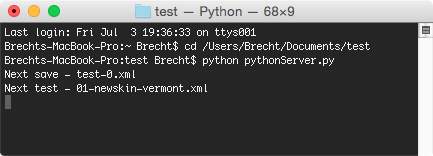
\includegraphics[width=.75\textwidth]{pythonServer.png}
	                \caption{Mac OS X: The Terminal window after going to the right folder (\texttt{cd [folder\_path]}) and running \texttt{pythonServer.py}.}
	                \label{fig:terminal}
	                \end{center}
	                \end{figure}

	        Alternatively, you can simply type \texttt{python} (follwed by a space) and drag the file into the Terminal window from Finder. % DOESN'T WORK YET
			
			You can leave this running throughout the different experiments (i.e. leave the Terminal open). 

		\subsubsection{Windows}
		
			Simply double click the Python script \texttt{pythonServer.py} in the folder you downloaded. 
			
			You may see a warning like the one in Figure \ref{fig:warning}. Click `Allow access'. 
			
			\begin{figure}[htbp]
	                \begin{center}
	                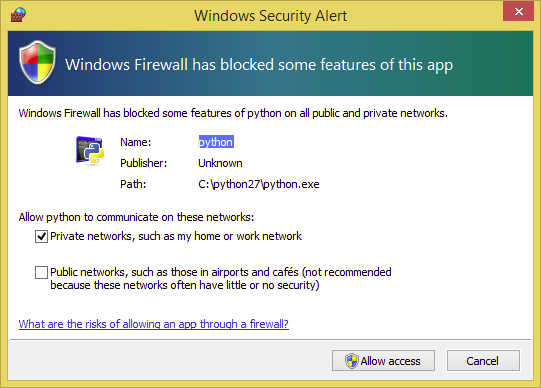
\includegraphics[width=.6\textwidth]{warning.png}
	                \caption{Windows: Potential warning message when executing \texttt{pythonServer.py}.}
	                \label{fig:warning}
	                \end{center}
	                \end{figure}
	                
	                The process should now start, in the Command prompt that opens - see Figure \ref{fig:python}. 
	                
	                \begin{figure}[htbp]
	                \begin{center}
	                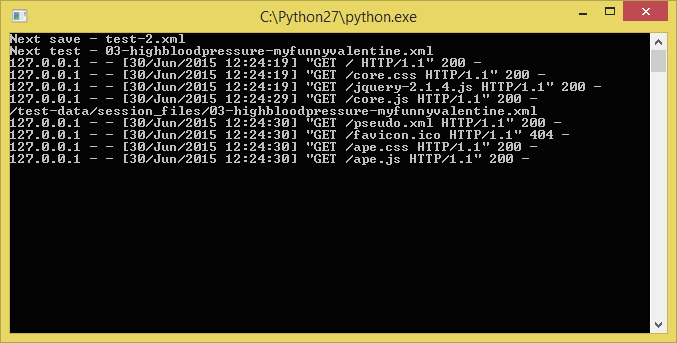
\includegraphics[width=.75\textwidth]{python.png}
	                \caption{Windows: The Command Prompt after running \texttt{pythonServer.py} and opening the corresponding website.}
	                \label{fig:python}
	                \end{center}
	                \end{figure}
	                
	                You can leave this running throughout the different experiments (i.e. leave the Command Prompt open). 
		
		
\clearpage
	\subsection{Sample rate}
		Depending on how the experiment is set up, audio is resampled automatically (the Web Audio default) or the sample rate is enforced. In the latter case, you will need to make sure that the sample rate of the system is equal to the sample rate of these audio files. For this reason, all audio files in the experiment will have to have the same sample rate. 

		Always make sure that all other digital equipment in the playback chain (clock, audio interface, digital-to-analog converter, ...) is set to this same sample rate.
		
		\subsubsection{Mac OS X}
			To change the sample rate in Mac OS X, go to \textbf{Applications/Utilities/Audio MIDI Setup} or find this application with Spotlight. Then select the output of the audio interface you are using and change the `Format' to the appropriate number. Also make sure the bit depth and channel count are as desired. 
			If you are using an external audio interface, you may have to go to the preference pane of that device to change the sample rate. 
		
		\subsubsection{Windows}
			To change the sample rate in Windows, right-click on the speaker icon in the lower-right corner of your desktop and choose `Playback devices'. Right-click the appropriate playback device and click `Properties'. Click the `Advanced' tab and verify or change the sample rate under `Default Format'.    % NEEDS CONFIRMATION
			If you are using an external audio interface, you may have to go to the preference pane of that device to change the sample rate. 
		 
				
		
	\subsection{Setting up a participant}
		
		\subsubsection{Instructions} % EXAMPLE?
			Before each test, show the instructions below or similar and make sure it is available to the subject throughout the test. Make sure to ask whether the participant has any questions upon seeing and/or reading the instructions. 
			
			\begin{itemize}
			\item You will be asked for your name (``John'') and location (room identifier). 
			\item An interface will appear, where you are asked to 
			\begin{itemize}
				\item click green markers to play the different mixes;
				\item drag the markers on a scale to reflect your preference for the mixes;
				\item comment on these mixes, using text boxes with corresponding numbers (in your \textbf{native language});
				\item optionally comment on all mixes together, or on the song, in `General comments'. 
			\end{itemize}
			\item You are asked for your personal, honest opinion. Feel free to use the full range of the scale to convey your opinion of the various mixes. Don?t be afraid to be harsh and direct. 
			\item The markers appear at random positions at first (which means some markers may hide behind others). 
			\item The interface can take a few seconds to start playback, but switching between mixes should be instantaneous. 
			\item This is a research experiment, so please forgive us if things go wrong. Let us know immediately and we will fix it or restart the test.  
			\item When the test is finished (after all songs have been evaluated), just call the experimenter, do NOT close the window.  
			\item After the test, please fill out our survey about your background, experience and feedback on the test. 
			\item By participating, you consent to us using all collected data for research. Unless asked explicitly, all data will be anonymised when shared. 
			\end{itemize}

		
		\subsubsection{The test}
			To start the test, open the browser and type 
			
			\texttt{localhost:8000}
			
			and hit enter. The test should start (see Figure \ref{fig:test}). 
			
			\begin{figure}[htb]
                        \begin{center}
                        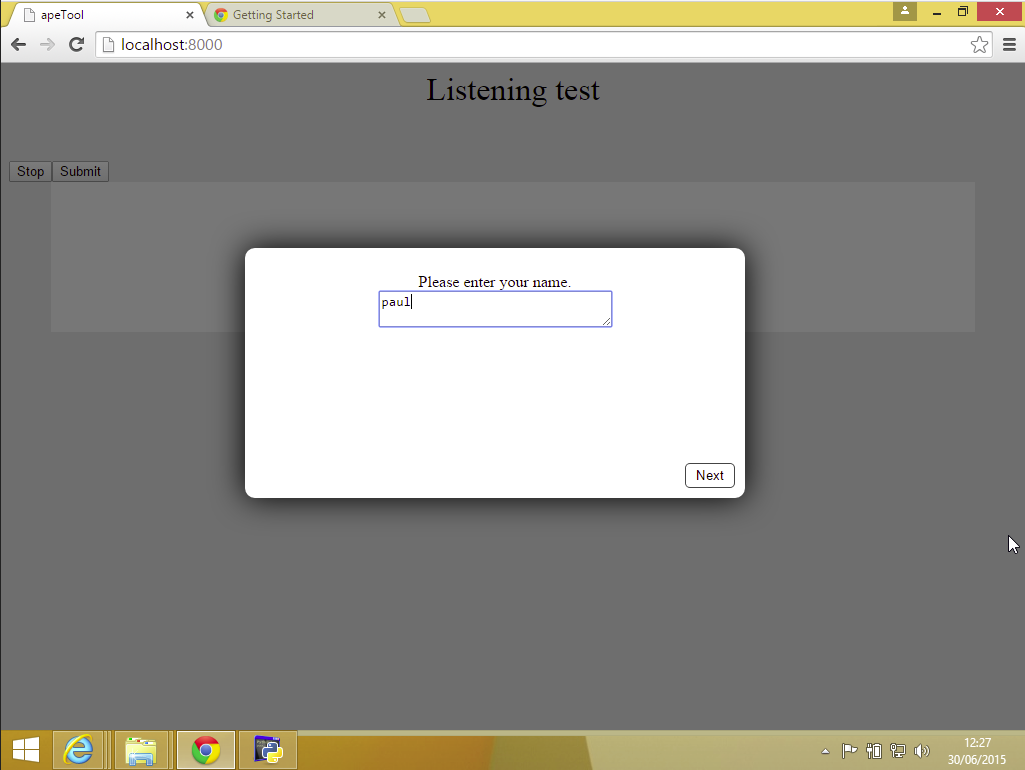
\includegraphics[width=.8\textwidth]{test.png}
                        \caption{The start of the test in Google Chrome on Windows 7.}
                        \label{fig:test}
                        \end{center}
                        \end{figure}
                        
            If at any point in the test the participant reports weird behaviour or an error of some kind, or the test needs to be interrupted, please notify the experimenter and/or refer to Section \ref{sec:troubleshooting}. 
			
			When the test is over (the subject should see a message to that effect, and click `Submit' one last time), the output XML file containing all collected data should have appeared in `saves/'. The names of these files are `test-0.xml', `test-1.xml', etc., in ascending order. The Terminal or Command prompt running the local web server will display the following file name. If such a file did not appear, please again refer to Section \ref{sec:troubleshooting}. 
			
			It is advised that you back up these results as often as possible, as a loss of this data means that the time and effort spent by the subject(s) has been in vain. Save the results to an external or network drive, and/or send them to the experimenter regularly. 
			
			To start the test again for a new participant, you do not need to close the browser or shut down the Terminal or Command Prompt. Simply refresh the page or go to \texttt{localhost:8000} again. 
			
			
		\subsubsection{Survey}
			The tool allows for embedded questions before and after each page, and before and after the whole test. If these do \underline{not} include survey questions (about the participant's background, demographic information, and so on) make sure to ask the participant to complete the survey immediately after the test. Above anything else, this decreases the likelihood that the survey goes forgotten and the experimenters do not receive the data in time. 
	
\clearpage
	\subsection{Troubleshooting} \label{sec:troubleshooting}
		Thanks to feedback from using the interface in experiments by the authors and others, many bugs have been caught and fatal crashes due to the interface (provided it is set up properly by the user) seem to be a thing of the past. 
		However, if things do go wrong or the test needs to be interrupted for whatever reason, all data is not lost. In a normal scenario, the test needs to be completed until the end (the final `Submit'), at which point the output XML is stored in the \texttt{saves/}. If this stage is not reached, open the JavaScript Console (see below for how to find it) and type 

		\texttt{createProjectSave()}

		and hit enter. This will open a pop-up window with a hyperlink that reads `Save File'; click it and an XML file with results until that point should be stored in your download folder. 
		
		Alternatively, a lot of data can be read from the same console, in which the tool prints a lot of debug information. Specifically:
        	\begin{itemize}
            	\item the randomisation of pages and fragments are logged;
            	\item any time a slider is played, its ID and the time stamp (in seconds since the start of the test) are displayed;
            	\item any time a slider is dragged and dropped, the location where it is dropped including the time stamp are shown; 
            	\item any comments and pre- or post-test questions and their answers are logged as well. 
        	\end{itemize}

		You can select all this and save into a text file, so that none of this data is lost. You may to choose to do this even when a test was successful as an extra precaution. 

		\subsubsection{Opening the JavaScript Console}
            \begin{itemize}
                \item In Google Chrome, the JavaScript Console can be found in \textbf{View$>$Developer$>$JavaScript Console}, or via the keyboard shortcut Cmd + Alt + J (Mac OS X). 
                \item In Safari, the JavaScript Console can be found in \textbf{Develop$>$Show Error Console}, or via the keyboard shortcut Cmd + Alt + C (Mac OS X). Note that for the Developer menu to be visible, you have to go to Preferences (Cmd + ,) and enable `Show Develop menu in menu bar' in the `Advanced' tab. 
                \item In Firefox, go to \textbf{Tools$>$Web Developer$>$Web Console}, or hit Cmd + Alt + K. 
            \end{itemize}

\clearpage
\section{Listening test: remote}

	(TBA)

\clearpage
\bibliographystyle{ieeetr}
\bibliography{ListeningTestInstructions}{}

\end{document}  